%!TEX root = ../main.tex

\gls{FPGA}-based \glspl{TDC} offers many benefits and advantages, but they also face several challenges. One significant problem is the high nonlinearity of the carry units in \gls{FPGA} devices due \gls{PVT} variations. The delay units of \gls{ASIC}-based \gls{TDC} also suffer from \gls{PVT} variations. However, addressing nonlinearities in \glspl{FPGA} cannot be done by using the same methods employed in \gls{ASIC} platforms since the resources available in \gls{FPGA} devices are predetermined from the start.

Over the years, various solutions to compensate the impact of \gls{PVT} variations on delay units in both \gls{ASIC} and \gls{FPGA} platforms has been proposed. In \gls{ASIC}-based \gls{TDC}, analog \gls{DLL} architectures are commonly used. Figure~\ref{fig:dll} shows the basic block diagram of a typical analog \gls{DLL}. This architecture consists of a phase detector, a charge pump, a loop filter and a \gls{VCDL}. Its operating principle is based on the detection of environmental changes and adjustment of the control voltage to maintain a constant delay of the delay cells in the \gls{VCDL}, regardless of \gls{PVT} variations. In~\citep{dll_2009} a \gls{DLL} architecture implemented in 0.35 \textmu m digital \gls{CMOS} technology achieved a temperature drift of less than 0.4~ps/\textdegree C over a range from -40~\textdegree C to +60~\textdegree C. Using the same \gls{CMOS} technology, \Citep{dll_2005} reported a temperature drift of below 0.05~ps/\textdegree C.

\begin{figure}[ht!]
	\centering
	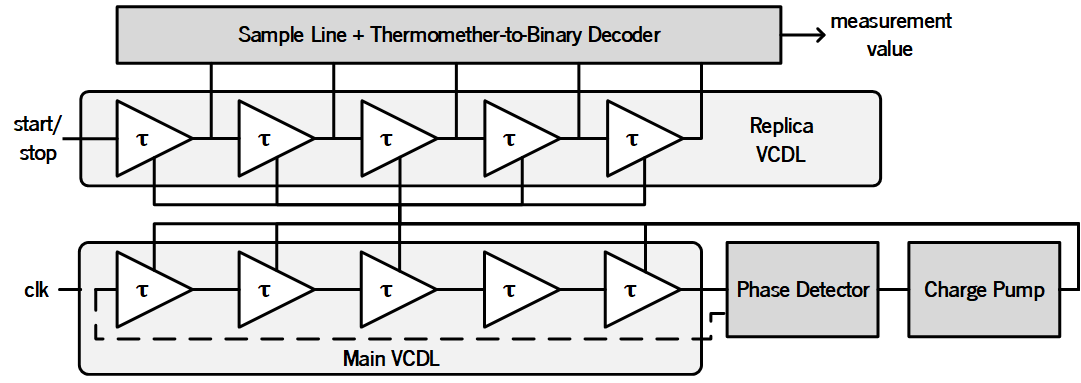
\includegraphics[width=.8\textwidth]{img/02_StateofArt/dll.png}
	\caption{General DDL architecture block diagram (adapted from \citep{addll_review}).}
	\label{fig:dll}
\end{figure}

Analog \gls{DLL} have high power consumption, long lock times and require large area. To overcome these limitations, improvements aimed at replacing analog components began to emerge. Semi-digital \glspl{DLL} replace the charge pump and loop filter with a counter and a \gls{DAC}, but they still use a \gls{VCDL}. In \glspl{ADDLL}, the \gls{VCDL} is replaced with a \gls{DCDL}, eliminating the need for a \gls{DAC}. The counter digitally controls the \gls{DCDL} to reach a lock state. The optimal value of the counter must be continuous tracked to compensate the phase drift due \gls{PVT} in the lock state. Compared to analog \glspl{DLL}, \glspl{ADDLL} have faster locking times, easier migration, higher power efficiency, and improved tolerance to \gls{PVT} variations. In~\citep{addll_res}, an \gls{ADDLL} implemented in 55~nm \gls{CMOS} technology achieved a 10.7~ps resolution while maintaining stable resolution with \gls{PVT} variations.

Different approaches to compensate for \gls{PVT} variations in \gls{FPGA}-based \glspl{TDC} can be found in the literature. However, despite their differences, they all use calibration tables (histograms/\glspl{LUT}) to achieve this compensation. \citet{temperature_coeffients} performed bin-by-bin calibrations at different temperatures to determine the temperature coefficient of the carry chain. These calibrations are performed for both a single-chain \gls{TDL} and a \gls{WU} \gls{TDL}. Based on the results, the authors developed a simplified temperature correction scheme that uses a dedicated correction channel to measure the temperature coefficient and correct the fine time result for all \gls{TDC} channels. The experimental results show that the \gls{TDC} has a 21~ps precision and is able to operate over a wide ambient temperature range from 0~\textdegree C to 60~\textdegree C.

\citet{pvt_offset} implemented an eight-channel, 20 carry-chains \gls{TDL}, analyzed the temperature-dependent delay variation function, and design an on-board cancel to ensure stable performance over a wide temperature range. This canceler is capable of effectively correct the delay offset over temperature for the carry chain as well as for the signal transmission path. The block diagram of the proposed offset canceler is shown in figure~\ref{fig:offset_canceller}. A temperature sensor is located near the \gls{FPGA} chip to measure the operating temperature for both the \gls{FPGA} and the signal transmission path. The \gls{INL} data of all the \gls{TDC} channels is stored in the \gls{INL} \gls{LUT}. \gls{INL} error and chain delay offset of the encoder outputs from \textit{N} carry chains are corrected in parallel by the offset canceler. After the chain delay offset is corrected, the data from multiple carry chains are averaged, and then the transmission delay is also corrected. To test the performance of the \gls{TDC} with offset canceler, the system was tested at temperatures raising from −20~\textdegree C to +60~\textdegree C with a rate of 1~\textdegree C per minute. The use of offset correction allowed for a significantly improved resolution of 4.4~ps, compared to 9.3~ps without offset correction. Additionally, a precision of 3.5~ps for 20 carry-chains was obtained. The approach just presented uses multiple chain measurements which are averaged to compensate \gls{PVT} variations. This approach requires calibrations \glspl{LUT} for each chain and for the delay between chains before averaging, resulting in the need for additional calibration steps to ensure accuracy. In contrast, a multiple-chain \gls{TDL} (as presented in subsection~\ref{sub:tapped_delay_lines}) allows to reduce the impact of temperature fluctuations on the precision, and only requires a single \gls{LUT} for the equivalent chain, eliminating the need for multiple \glspl{LUT} and additional calibration steps. The bin size of plain chain is affected by temperature fluctuations, which cannot be reduced by averaging. However, by segmenting the bin size variation of the plain chain, the equivalent chain becomes insensitive to temperature fluctuations, eliminating the need for a dedicated temperature. The resolution of the 10 chain \gls{TDL} implemented in~\citep{pvt_mc} is stable with a temperature coefficient of 0.0002~ps/\textdegree C over an operating temperature range from 25~\textdegree C to 70~\textdegree C.

\begin{figure}[ht!]
	\centering
	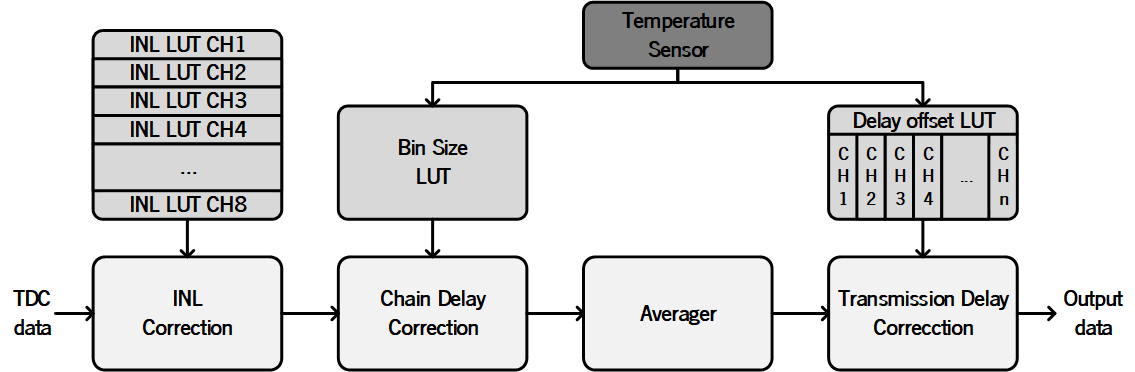
\includegraphics[width=.8\textwidth]{img/02_StateofArt/offset_canceller.png}
	\caption{Block diagram of the offset canceler (adapted from \citep{pvt_offset}).}
	\label{fig:offset_canceller}
\end{figure}

In \citeyear{pvt_ro}, \citet{pvt_ro} proposed a novel method of compensating the temperature effect on the delay line. This design uses a \acrlong{RO}, consisting of 31~NOT and one~AND gates, placed next to the tapped delay line. Two calibration tables are used to calibrate automatically and online in the hardware. The frequency of the \gls{RO} is measured and compared with the frequency acquired at the beginning of the measurements. The compensation is performed by scaling the \acrlong{LUT} coefficients evaluated in the bin-by-bin calibration phase, \textit{T(i)\textsubscript{bybline}}, according to the equation~\ref{eq:pvt_ro}, where \textit{f\textsubscript{bybline}} is the frequency counter of bin-by-bin calibration and \textit{f\textsubscript{online}} is the frequency counter of online calibration. The results showed that the frequency count value decreases linearity with the increase of temperature, about 4~\textdegree C. To test the online temperature compensation circuit, the operating temperature is increased from 30~\textdegree C to 70~\textdegree C. The \gls{TDC} \gls{RMS} precision without calibration increases linearly with the increase of temperature, by about 0.6~ps/\textdegree C, whereas the \gls{TDC} with calibration circuit remains below 19~ps.

\begin{equation}
	T(i)_{online} = \frac{f_{bybline}}{f_{online}} * T(i)_{bybline}
	\label{eq:pvt_ro}
\end{equation}

Currently, the calibration of \glspl{TDL} mainly depends on the calibration module built in \glspl{FPGA} based on code density tests. These tests have a long calibration time, which can worsen the system's dead time. Additionally,the problems cause by \gls{PVT} variations often require frequent calibrations to maintain working accuracy, which can further aggravate the aforementioned problems. To address these problems, \citet{bin_by_bin_calibration_neural_network} proposed a novel \gls{TDL} calibration method based on a neural network. The method uses an on-chip calibration module on an \gls{FPGA} and a network calibration module on a host computer to collect delay time data and corresponding temperature information for each \gls{TDL} bin. The delay time and temperature data are used as raw data samples for training, and the trained network structure is used as the result of the network calibration module. Based on this paper, it can be concluded that a neural network calibration module built on a host computer can be used on different \gls{FPGA} platforms and can compensate the influence of temperature on \gls{TDC}.